\section{Experiments}
\subsection{Experimental Setup}


I verify the proposed PINN methods on generated dataset, and FDTD methods with hybrid and pure MPI strategies
on the server with two Intel (R) Xeon (R) Platinum 9242 CPU nodes (96 cores per node) and $4$ NUMA nodes per node.
While the dataset is using \texttt{std::m19937} STL random device with given seed $42$ \cite{STL:RANDOM_SEED}.
The PINN models I mentioned are trained using train-from-scratch strategy, and maximin number of training times is $1'000'000$ epochs.
In the setting of learning rate and optimizer, I chose to use Adam with constant learning speed $10^{-3}$.
The details of PDEs are determined in previous section \ref{SEC:Specific_Form}.  

\paragraph{Compiling}
Compiling the program is also a critical important processes.
I chose to use the macros for defining the scale of problems in advance, this is because the compiler will 
have more aggressive optimizations if it knows more predefined parameters.

\paragraph{Running}
For finely manipulate the resource allocation on cluster, following command line \ref{LST:mpirun} is used for this 
the script arguments \texttt{rsc} stands for the resource type such as \texttt{numa}, \texttt{node} and \texttt{socket},
\texttt{--report-bindings} is a error message, for showing the details of threads and CPUs tasks allocated on cluster.
\begin{lstlisting}[
  style=customCpp,
  caption={main command line for launching program on cluster},
  label={LST:mpirun}]
    mpirun --map-by ppr:$ppr:$rsc:pe=$threads --report-bindings <executable> <arguments>
\end{lstlisting}
and \texttt{threads} means the number of threads per resource. The \texttt{ppr} is the number of CPU tasks per resource.
The last \texttt{<argument>} is command line arguments for the program, which is designed by programmer. 
In this case, I designed three type of arguments
\begin{enumerate}
  \item \texttt{-S, -s} Strategy, for specifying the pure mpi, hybrid 0 or 1 strategy.
  \item \texttt{-F, -f} file name, if this argument is defiend, the results will be stored in the file.
  \item \texttt{-H, -h} Helper message, the usage information.
  \item \texttt{-V, -v} Showing the version of program.
\end{enumerate}



\subsubsection{Computational Topology}
The computational topology is critically important when we are programming parallel PDEs solver softwares.
Put the strongly speed-dependent data into the slow memory could make entire program slower.

\paragraph{Cluster}
The cluster we are using for this project is \texttt{Callan} \cite{Callan_TCD} which has 
$2$ CPUs per compute node, and each CPU has $32$ cores with single thread. 
The Non-Uniform Memory Access (NUMA) nodes are layout as following 
\begin{figure}[htbp]
  \centering
  \begin{tikzpicture}[scale=0.8, transform shape]
    \node[anchor=south west,inner sep=0] (image) at (0,0) {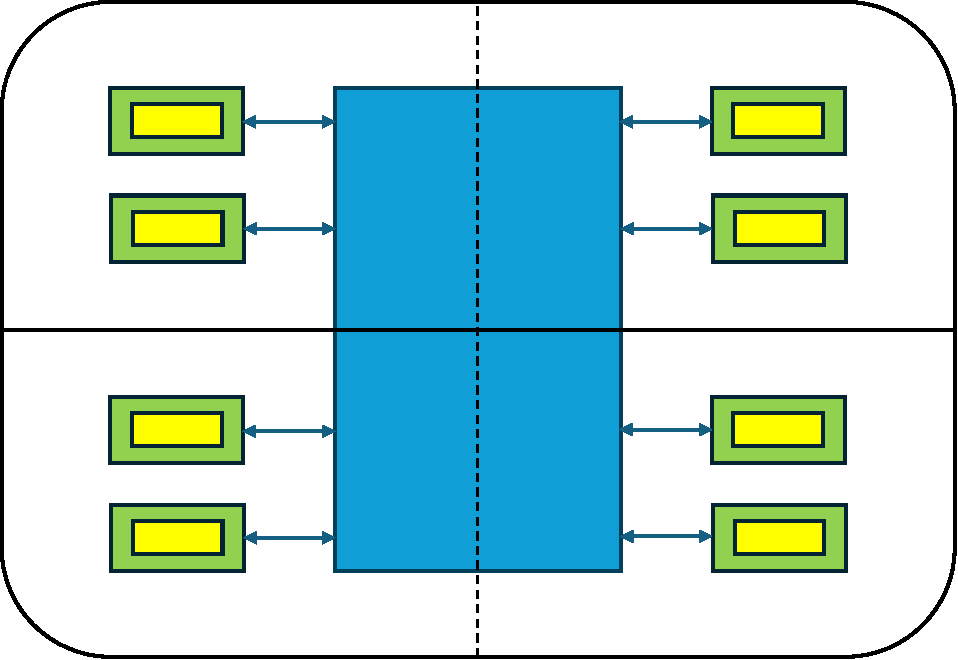
\includegraphics[width=0.5\textwidth]{figure/FIG_Topology_9242.pdf}};
    % \node[anchor=south west,inner sep=0] (image) at (0,0) {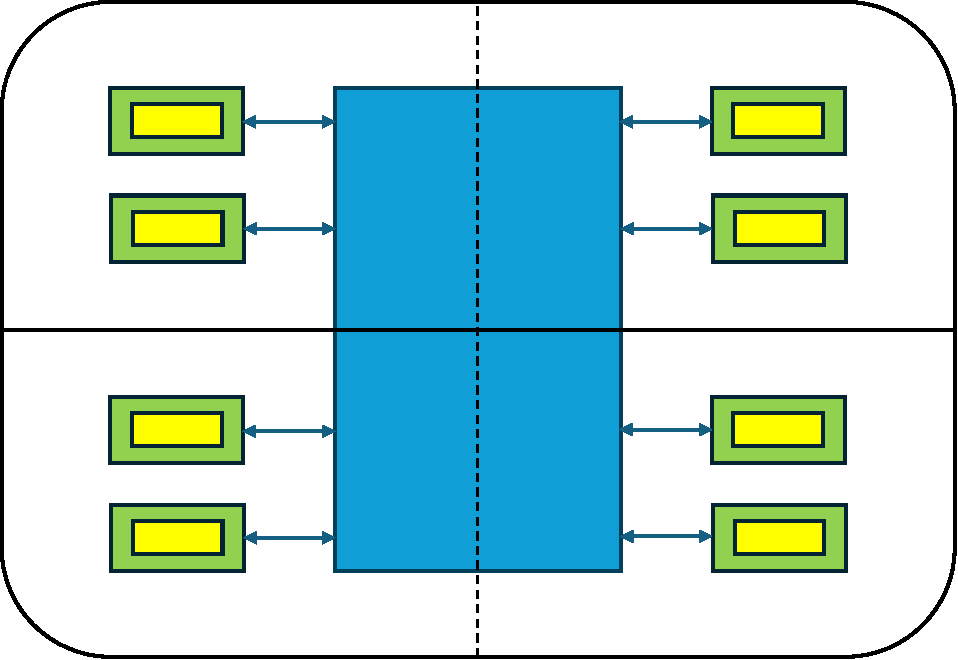
\includegraphics[width=0.58\textwidth]{figure/FIG_Topology_9242.pdf}};     /// overleaf
    \begin{scope}[x={(image.south east)},y={(image.north west)}]
        % \draw[help lines, step=1em] (-1em,-1em) grid (30em,20em);    
        % % Draw axes
        % \draw[dashed,->] (-1em,0) -- (30em,0) node[right] {x};
        % \draw[dashed,->] (0,-1em) -- (0,20em) node[above] {y};

      \node at (12em,18em) {$2$ $Scokets$};

      \node at (4.5em,1em) {$DDR4$};
      \node at (19.5em,1em) {$DDR4$};

      \node at (4.5em, 15em) {$DDR4$};
      \node at (19.5em,15em) {$DDR4$};

      \node at (12em,13em) {Hyper-threads};
      \node at (12em,5.5em) {Hyper-threads};

      \node at (12em,11em) {$48$ $CPUS$};
      \node at (12em,3.5em) {$48$ $CPUS$};
    \end{scope}
  \end{tikzpicture}
  \caption{NUMA topology of single node on Cluster}
  \label{FIG_Topology_Callan}
\end{figure}
Accessing the other NUMA node's memory reduces the bandwidth and also the latency,
though the bandwidth is commonly high enough, the latency can increase by 
$~30\%$ to $~400\%$ \cite{NUMA_Latency_TCD}. 
This latency becomes dangerous when writing shared memory parallel programs.


\subsection{Comparison on single node}
On single node, the CPUs are connected by high-bandwidth, low-latency internal bus which is faster than connection between nodes.
However, for the $4$ total NUMA nodes per compute node, memory accessing between them has higher latency than cache.
Thus, the first tests set were run on the platform with single node, to evaluate the parallelistic performance of heat equation on 2 and 3 dimension spaces with 
3 strategies.


\subsubsection{Strong Scaling}
Figure \ref{FIG:Benchmark:PURE_MPI} visualizes the comparison of my proposed parallelistic program using pure MPI on two dimension space heat euqation with 
the number of CPUs and various problem scales.
Overall, the more CPUs brings more performance among all scales from $512^2$ to the $32'768^2$ but can not break the speedup limits.
Compared with large scale bigger than $4096^2$, the light problems has less speedup as the number of CPUs increases.
By seeing the trend of speedup ratios drop as the CPU gets more, 
the trend can be readily discovered which is the as the scale of problems gets larger, the latter it will have performance-dropping.
Once the problem size is large enough, ($4096^2$ and larger), the solvers can get the more benefits from more CPUs.

\begin{figure}[htbp]
  \centering
  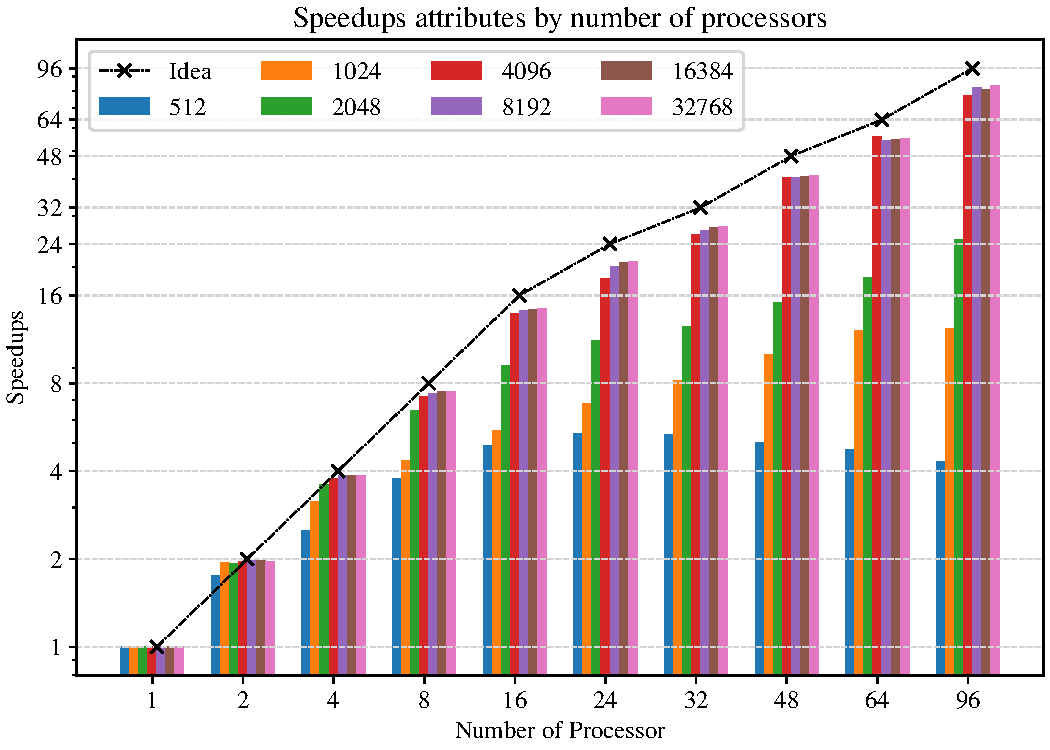
\includegraphics[width=0.6\textwidth]{figure/FIG_Benchmark_pure_mpi.pdf}
  \caption{
    Comparison of speedup ratios of strong scaling tests of pure MPI parallelized program. 
    The investigated problem scales are the power of $2$, exponents ranging from $9$ to $15$.
    The number of CPUs are also set as power of $2$, with additional numbers $24$, $48$ and $96$ matched the topologies of CPU.
  }
  \label{FIG:Benchmark:PURE_MPI}
\end{figure}

On the other hand, I also include some unconventionaly number of CPUs in scaling tests such as $24$, $48$ and $96$ for comparison. and 
the results are also shown in the figure \ref{FIG:Benchmark:PURE_MPI}.
From this figure, it is hard to tell the difference of these where it ought to indicate some information about its NUMA structure.
This is because the MPI communication does not strongly effected by memory structure, while the hybrid does.
Figure \ref{FIG:Benchmark:Hybrid} shows the difference, the hybrid strategy brings lower performance with small scale across all CPUs and 
approximately identical in the large scale cases.
The most visible change in figure \ref{FIG:Benchmark:Hybrid_0} is that the speedup ratio of problem with scale $4096^2$ 
exceded the limits on $4$, $8$ and $16$ CPUs which is $1$, $2$, $4$ threads of each MPI process.
We can also see that when the number of threads is $8$ and $4$ MPI processes, the performances on large scale is better than pure MPI parallelism.

\begin{figure}[htbp]
  \centering
  \subfigure[No overlapping comm./comp.]
  {
    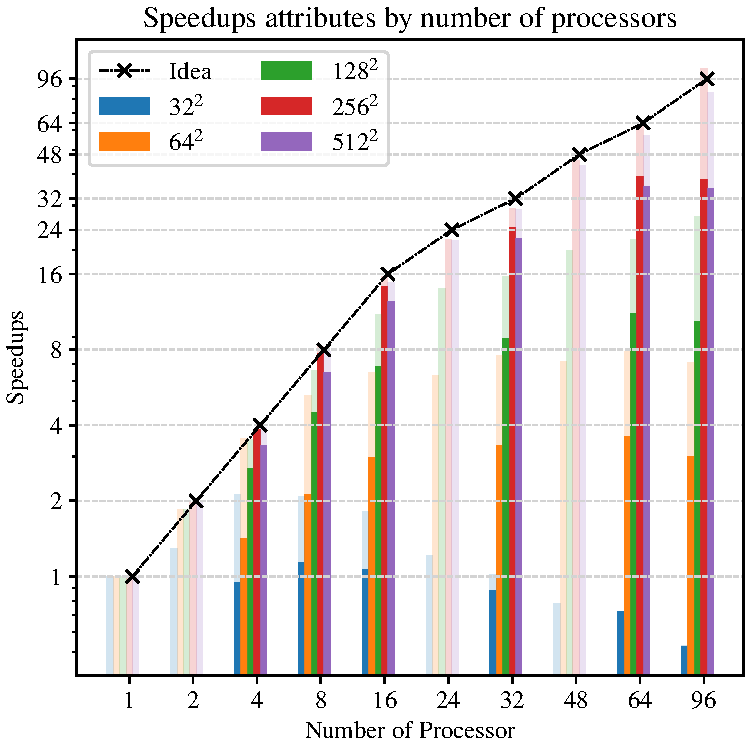
\includegraphics[width=0.47\textwidth]{figure/FIG_Benchmark_hybrid_0.pdf}
    \label{FIG:Benchmark:Hybrid_0}
  }
  \hfill
  \subfigure[With overlapping comm./comp.]
  {
    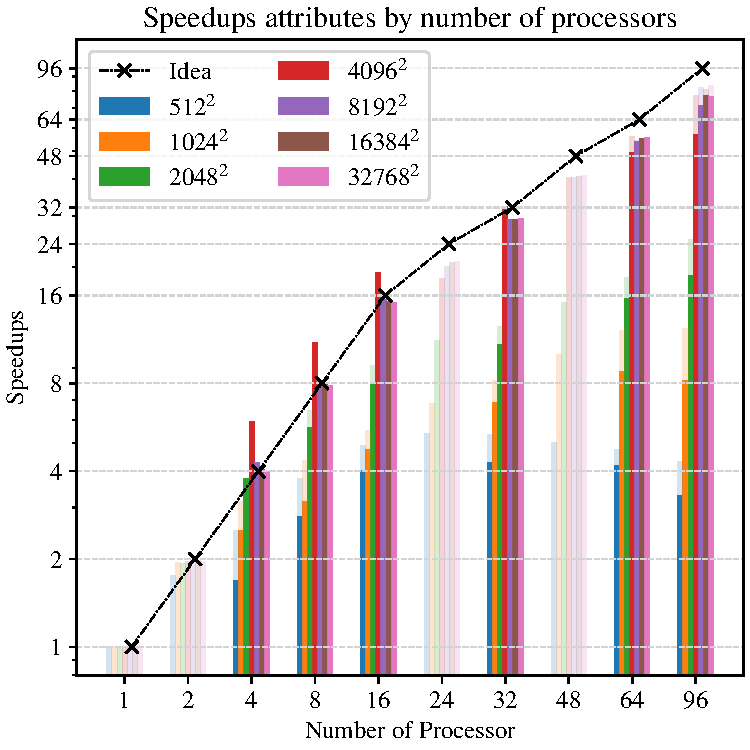
\includegraphics[width=0.47\textwidth]{figure/FIG_Benchmark_hybrid_1.pdf}
    \label{FIG:Benchmark:Hybrid_1}
  }
  \caption{
    Comparison of speedup ratios of strong scaling tests of mater-only parallelized program with overlapping and no overlapping of computation and communication.  
    The vague background is the results of pure MPI parallelization from figure \ref{FIG:Benchmark:PURE_MPI} and problems sclaes are identical as well.
    The number of threads are set to $1$, $2$, $4$, $8$, $16$, and $24$, 
    tasks per CPU are $1$, $2$ and $4$.
  }
  \label{FIG:Benchmark:Hybrid}
\end{figure}

For the other funneled hybrid parallelization, the figure 
            \ref{FIG:Benchmark:Hybrid_1} 
in the appendix shows the details of results,
this strategy has nearly idential performance of master only with no overlapping on large problem scales.
However, the behaviour of it on small scales has a different pattern.
This indicates that the overlappings of computation and communication are not as good as previous one, which means the overload management is not 
well on these tests.


\paragraph{Superliner Speedup}
Conventionally, the actuall speedup won't excedes the theoratical predictions of Amdalh's law.
However, the scaling of two hybrid programs did exceded the limits but exclusively on the problem scale $4096^2$ and $1$ to $8$ threads of each $4$ MPI processes.
Considering the details of the CPU used for these tests, 
\begin{itemize}
  \item It has $4$ NUMA node per CPU and once of which has $12$ CPUs with $2$ threads.
  \item It has \texttt{32KB} L1 data and L1 instruction cache, \texttt{1024KB} L2 cache and \texttt{36608KB} L3 cache.
\end{itemize}
The data type for this solver is \texttt{Double} which takes $8$ bytes, and $4096^2$ \texttt{Double} numbers takes 128 \texttt{MB} to store.
In the case of $4$ MPI processes, each process own a quater of number which uses 32 \texttt{MB} for handling sub-problems.
On the other hand, the L3 cache is 36608 \texttt{KB} = 35.75 \texttt{MB} which is just bigger than the sub-problem scale 32 \texttt{MB}.
When the problem size gets larger, such as $8096^2$ which takes 128 \texttt{MB} to store the sub-problem. 
In such case, the L3 case is no longer able to hold it, thus part of the numbers will be stored in the DDR4 memories which is lower bandwidth and higher latency than cache.
Moreover, due to the CPU enables hyper-threading, a NUMA node actually holds $12$ CPUs, which makes the 
superlinear speedup disappear when the threads is 16 and 24.

% \begin{figure}[htbp]
%   \centering
%   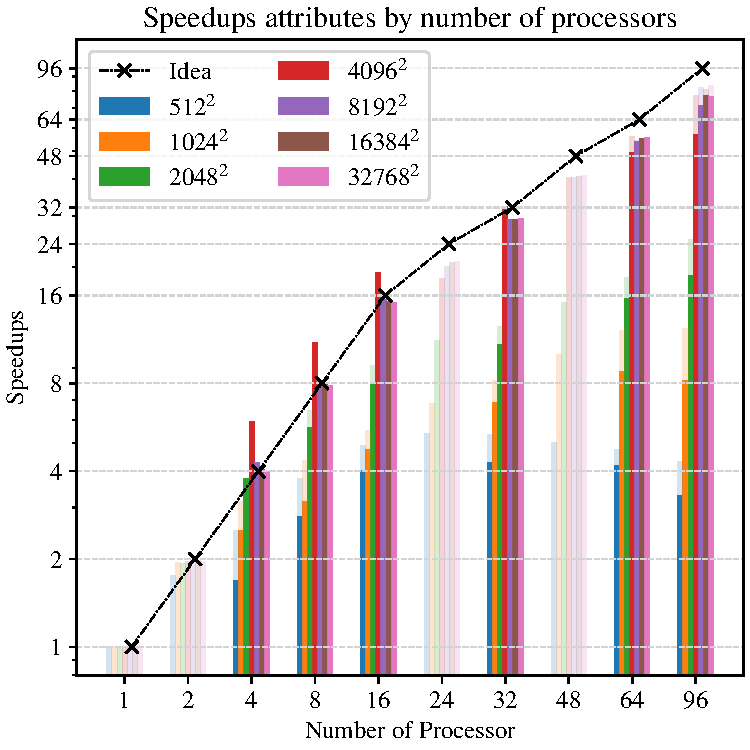
\includegraphics[width=0.7\textwidth]{figure/FIG_Benchmark_hybrid_1.pdf}
%   \caption{<caption>}
%   \label{FIG:Benchmark:Hybrid_1}
% \end{figure}

% \begin{figure}[htbp]
%   \centering
%   \subfigure[Grid sizes: 150*45*40/25*33*40.]{
%       \includegraphics[width=0.45\textwidth]{weak.png}
%       \label{fig:weak_scaling_1}    
%   }
%   \hfill
%   \subfigure[Grid sizes: 300*90*80/50*65*80]{
%       \includegraphics[width=0.48\textwidth]{weak_scaling_2_efficiency_comparison.png}    
%       \label{fig:weak_scaling_2}
%   }
%   \caption{
%       Weak scaling tests of Cartesian / Cylinder equation with same problem scale on $1$, $2^2$, $3^3$, $4^3$ processors.
%   }
%   \label{fig:weak_scaling}    
% \end{figure}

\subsubsection{Weak Scaling}\label{SSS:Weak_Scaling:SingleNode}

Table \ref{TAB:Benchmark:Weak_PURE_MPI} lists the weak scaling comparison of three different parallel strategies.
Overall, both three strategies have good weak scaling results across all problem sizes.
For example, according to the Gaustafsson's Law \ref{THEO:GaustafssonLaw}, the program using
overlapped strategy has sequential fraction 
$$f_s = \frac{49.989 - 64}{1-63} \approx 0.222$$
on the problem scale $4096^2$ with 64 CPUs
and $f_s \approx 0.147$ with 16 CPUs.
For the small size problems, like $512^2$, the pure MPI has significantly higher weak scaling efficiency comparing to the other two,
more specifically about $7.8\%$, $7.5\%$ higher in 64, 16 CPUs, and $22.5\%$ higher in 4 CPUs.
However, as the scale gets larger, this advantages gradually disappear and even worse than other two.
Especially when $4096^2$ on 16 and 64 cores, the forward leap of hybrid versions gets larger, about $34.4\%$ and $28.1\%$ higher than 
pure MPI respectively.

On the other hand, the superlinear speedup appears for the problem size with $512^2$ and $1024^2$ on 4 CPUs.
This is because the sub-problem for each CPUs only take 512 \texttt{KB} and 1024 \texttt{KB} to store, 
which is the L2 cache size of the Xeon Platinum 9242.
Thus the four processes could take the performance advantages of L2 cache individual for each CPU.
Once the problem size gets larger, such as $2048^2$, part of the problem will be allocated on L2 cache and other parts on L3 cache.
These memory allocations requires extra synchronization between cache accessing, which drop the performance down.
However, as the size gets to $4096^2$, the sub-problem will be fully make use of L3 cache, which require less synchronization of cache, 
the weak scaling goes up but we can not see the superlinear speedup again.

\begin{table}
  \caption{Weak Scaling on Single Node of 2D Heat Equation}
  \label{TAB:Benchmark:Weak_PURE_MPI}
  \begin{minipage}{\columnwidth}
    \begin{center}
      \footnotesize % overleaf
      \begin{tabular}{>{\bfseries}p{3cm} p{1.5cm} p{1.5cm} p{1.5cm} p{1.5cm} p{1cm}}
        \toprule
        \multirow{2}{*}{Strategy}     & \multirow{2}{*}{\bfseries Size} & \multicolumn{3}{c}{\bfseries  Number of CPUs}   & \multirow{2}{*}{\bfseries $f_p(\%)$}  \\
                                      &                                  & \bfseries 4   & \bfseries 16   & \bfseries 64  &                                       \\
        \midrule
        Pure MPI      & \multirow{3}{*}{$512^2$}      & 4.006  & 12.497  & 47.849                                         & 75.1 \\
        No Overlap    &                               & 2.876  & 11.206  & 42.754                                         & 67.0 \\
        With Overlap  &                               & 3.173  & 10.818  & 42.282                                         & 66.2 \\
        \midrule
        Pure MPI      & \multirow{3}{*}{$1024^2$}     & 3.838  & 9.304   & 33.707                                         & 53.2  \\
        No Overlap    &                               & 3.947  & 12.995  & 33.447                                         & 54.1 \\
        With Overlap  &                               & 4.024  & 12.932  & 33.361                                         &  54.0 \\
        \midrule
        Pure MPI      & \multirow{3}{*}{$2048^2$}     & 2.376  & 8.245   & 31.203                                         &  49.0\\
        No Overlap    &                               & 3.874  & 8.972   & 31.510                                         &  49.8 \\
        With Overlap  &                               & 3.740  & 8.989   & 31.430                                         &  49.7 \\
        \midrule
        Pure MPI      & \multirow{3}{*}{$4096^2$}     & 3.543  & 8.245   & 31.203                                         &  77.5\\
        No Overlap    &                               & 3.953  & 13.799  & 49.515                                         &  78.0\\
        With Overlap  &                               & 3.948  & 13.800  & 49.989                                         &  78.7 \\
        \bottomrule
      \end{tabular}
    \end{center}
    % \bigskip
    % \footnotesize\emph{Source:} This is source 
  \end{minipage}
\end{table}

Moreover, since Gaustafsson' theorem \ref{THEO:GaustafssonLaw} gives us a linear module for valuating the parallel problem.
Thus I chose to use the linear model from equation \ref{EQ:GaustafssonLaw} as a linear polymonimal fitting.
Considering the original point has to be on the line, which stantds for $f_s + f_p = 1$, 
I manually create an extended version of speedups by concatenate a inverse negative one to ensure their 
means are $0$ which makes the fitting line across the $(0,0)$. 
Eventually, the results of $f_p$ are shown in the table \ref{TAB:Benchmark:Weak_PURE_MPI} as well.
These fitting lines also indicate that the hybrid parallelized versions has more parallel fraction than pure MPI when the scale of problem gets larger than $512$,
which means that hybrid strategies reduced the cost of synchronization and brought higher efficiency.



\subsection{Comparison on multi-node}
Running programs on multi-node also utilized the command line \ref{LST:mpirun} to specify the resource allocation on cluster.
In this setup, I ran the tests on $4$ nodes with total $16$ NUMA nodes or $384$ CPUs, all other settings are maintained from the single-node tests.
\subsubsection{Strong Scaling}
Figure \ref{FIG:Benchmark:PURE_MPI_Multi_Node} demonstrates speedup ratio of all candidates for test and their relationships with the number of CPUs.
In the big picture, it is easy to determine that the small scale problems (smaller than $4096^2$) had pool speedup performances on these settings.
Especially for the $512^2$, $1024^2$ and $2048^2$, parallelization even brought worse performance in the end, which is 
strongly different from the big scales.
In the large scale problems, the most large two maintained good strong scaling performances at the end, but 
the pure MPI failed on launching the program when using $384$ processes.
Moeover, the problem with $4096^2$ numbers show superlinear speedup on $4$, $8$ and $16$ processes which 
is similar to single-node hybrid tests.
However, unlike gaining benefits from shared memory operations on single NUMA node, 
these superlinear speedup came from the node structure.
Where the pure MPI processes were allocated on four different CPU, which has individual CPU clock cycle.
Thus, the processes can behave like operating on shraed memory model.
\begin{figure}[htbp]
  \centering
  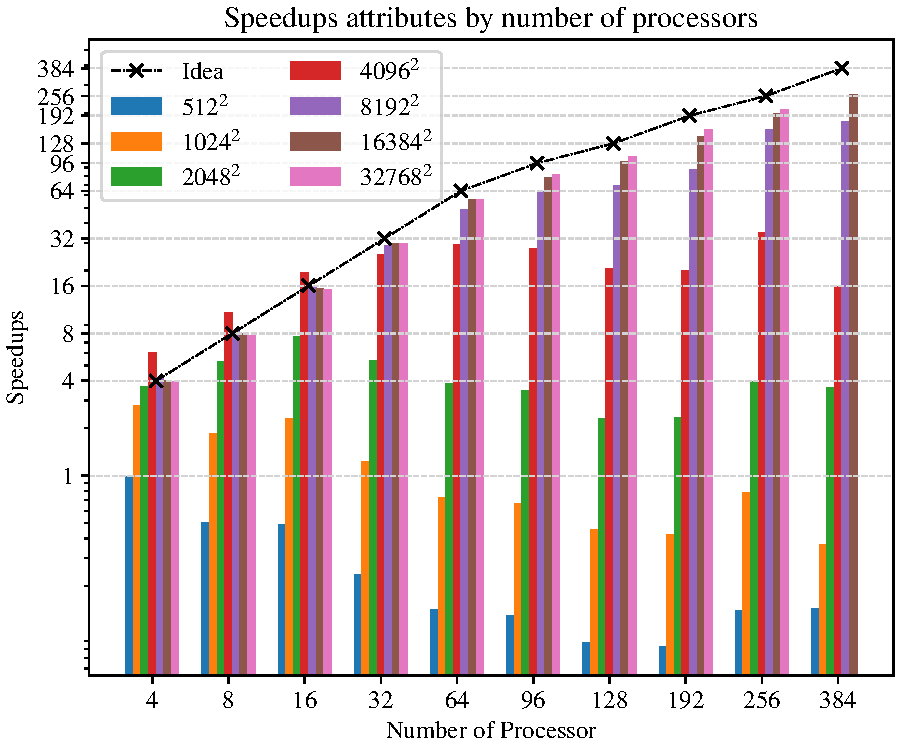
\includegraphics[width=0.55\textwidth]{figure/FIG_Benchmark_pure_mpi_multi_nodes.pdf}
  \caption{
    Comparison of speedup ratios of strong scaling tests of pure MPI parallelized program. 
    The investigated problem scales are the power of $2$, exponents ranging from $9$ to $15$.
    The number of CPUs are also set as power of $2$, with additional numbers $96$, $192$ and $384$ matched the topologies of CPU.
  }
  \label{FIG:Benchmark:PURE_MPI_Multi_Node}
\end{figure}
In addition, the patterns of the strong scaling are different from the Amdalh'S law \ref{THEO:Amdalh's law} demonstrates.
Which has may visible exceptional performance decreases, due to the topologies of CPUs, especially when using 
$32$, $48$ and $96$ CPUs per node.

On the other hand, 
based on comparison of the strong scaling speedup ratios and the amount of resources,
two hybrid versions performed better than pure MPI parallel and the 
results are shown in the figure \ref{FIG:Benchmark:Hybrid_Multi_Node}.
From the figure \ref{FIG:Benchmark:Hybrid_0_Multi_Node} and \ref{FIG:Benchmark:Hybrid_1_Multi_Node},
we could see that the superlinear speedup appears on the scale $4096^2$ and $8019^2$ which are effected by 
the previously mentioned two reasons, the high performance local NUMA node shared memory and individual CPU clock cycle.
More specifically, $8092^2$ \texttt{Double} numbers takes $512$ \texttt{MB} to store, $128$ \texttt{MB} on each node and $32$ \texttt{MB} per NUMA node,
which just fits the L3 cache size.

\begin{figure}[htbp]
  \centering
  \subfigure[No overlapping comm./comp.]
  {
    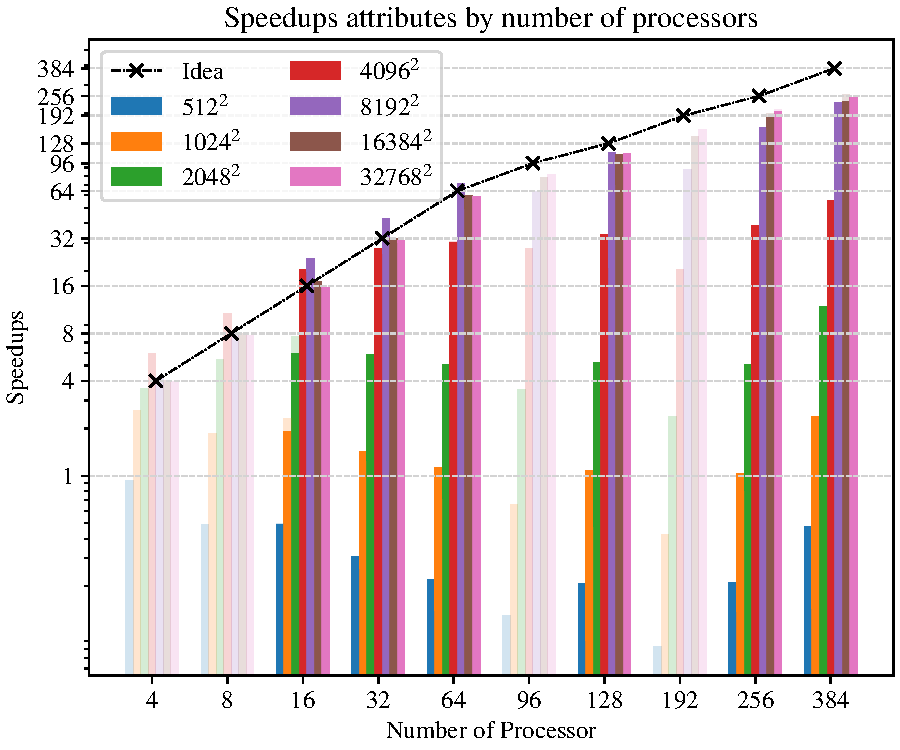
\includegraphics[width=0.47\textwidth]{figure/FIG_Benchmark_hybrid_0_multi_nodes.pdf}
    \label{FIG:Benchmark:Hybrid_0_Multi_Node}
  }
  \hfill
  \subfigure[With overlapping comm./comp.]
  {
    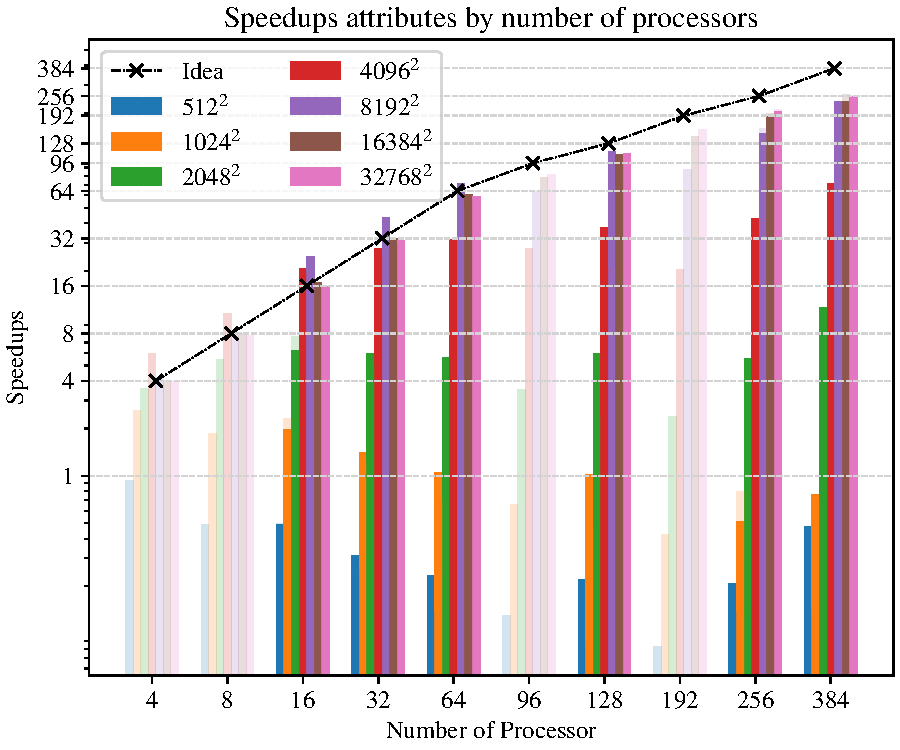
\includegraphics[width=0.47\textwidth]{figure/FIG_Benchmark_hybrid_1_multi_nodes.pdf}
    \label{FIG:Benchmark:Hybrid_1_Multi_Node}
  }
  \caption{
    Comparison of speedup ratios of strong scaling tests on $4$ nodes of 
    mater-only parallelized program with overlapping and no overlapping of computation and communication.  
    The vague background is the results of pure MPI parallelization from figure 
    \ref{FIG:Benchmark:PURE_MPI_Multi_Node} and problems sclaes are identical as well.
    The number of threads are set to $1$, $2$, $4$, $8$, $16$, and $24$, 
    tasks per CPU are $1$, $2$ and $4$.
  }
  \label{FIG:Benchmark:Hybrid_Multi_Node}
\end{figure}

As the amount of resources increase, the speedups are not increase as expected for all three parallel models.
However, hybrid parallel models were successfully launched on the $384$ CPUs, 
and also brought more performance for all tested number of CPUs.
These shows that the advantages of combination of shared memory programming and message-passing programming.

\subsubsection{Weak Scaling}

% PURE
% 512 48.185757348293464 [  3.29985789  10.37890476  25.99976339 124.37502699]
% 1024 49.30470677010394 [ 3.84763481 13.03676319 30.14287326]
% 2048 50.62289960989542 [ 3.7870875   9.17180313 32.01277006]
% 4096 80.22207174643209 [ 3.88441248 13.85932765 51.04086597]

% Hybrid 0
% 512 49.318336840965884 [  8.09445064  25.93147463 127.648308  ]
% 1024 69.80932598630608 [13.70192876 44.04014219]
% 2048 55.675781151306126 [13.93648546 34.36848416]
% 4096 83.806215053791 [15.31462331 53.15704013]

% Hybrid 1
% 512 45.51606462315708 [  8.38595555  27.12574758 116.95116903]
% 1024 69.93179786064245 [13.83401    44.09042189]
% 2048 55.86720303491557 [14.27434744 34.41421545]
% 4096 84.15726269711293 [15.29389611 53.40098918]
Table \ref{TAB:Benchmark:Weak_PURE_MPI_Multi_Node} lists the weak scaling comparison results of multi-node tests.
Overall, the hybrid models have better scaling speedup ratios than pure MPI model on the size larger than $512^2$.
Although the speedups of pure MPI model are better than hybrid models on $16$ CPUs with $2048^2$ problem size,
the hybrid model with no comm./comp. overlapping still have better performance when testing is running on $64$ and $256$ CPUs.
Controversially, the hybrid with no overlapping has better results comparing to the one with overlapping,
and we have opposite results when the scale gets larger.

On the other hand, similar to previous section \ref{SSS:Weak_Scaling:SingleNode}, the fraction of parallelizable is approximated by linder regression 
based on the model proposed in theorem \ref{THEO:GaustafssonLaw}.
As the table \ref{TAB:Benchmark:Weak_PURE_MPI_Multi_Node} lists results, the fraction of parallelizable increases as the size gets larger.
Moreover, the overlapping has the most large fraction then the model with no overlapping, and both of then are significantly larger than pure MPI model.

\begin{table}[htbp]
  \caption{Weak Scaling on Multi-node of 2D Heat Equation}
  \label{TAB:Benchmark:Weak_PURE_MPI_Multi_Node}
  \begin{minipage}{\columnwidth}
    \begin{center}
      \footnotesize % overleaf
      \begin{tabular}{>{\bfseries}p{3cm} p{1.5cm} p{1.5cm} p{1.5cm} p{1.5cm} p{1.5cm} p{1cm}}
        \toprule
        \multirow{2}{*}{Strategy}     & \multirow{2}{*}{\bfseries Size} & \multicolumn{4}{c}{\bfseries  Number of CPUs}   & \multirow{2}{*}{\bfseries $f_p(\%)$}  \\
                                      &                                 & \bfseries 4   & \bfseries 16   & \bfseries 64  & \bfseries 256  &                        \\
        \midrule
        Pure MPI      & \multirow{3}{*}{$512^2$}      & 3.300  & 10.379  & 26.000   & 124.375                                    & 48.2 \\
        No Overlap    &                               &   -    &  8.094  & 25.931   & 127.648                                    & 49.3 \\
        With Overlap  &                               &   -    &  8.386  & 27.126   & 116.951                                    & 45.5 \\
        \midrule
        Pure MPI      & \multirow{3}{*}{$1024^2$}     & 3.848  & 13.037  & 30.143   &   -                                        & 49.3 \\
        No Overlap    &                               &   -    & 13.702  & 44.040   &   -                                        & 69.8 \\
        With Overlap  &                               &   -    & 13.834  & 44.090   &   -                                        & 69.9 \\
        \midrule
        Pure MPI      & \multirow{3}{*}{$2048^2$}     & 3.787  & 9.172   & 32.013   &   -                                        & 50.6 \\
        No Overlap    &                               &   -    & 13.936  & 34.368   &   -                                        & 55.7 \\
        With Overlap  &                               &   -    & 14.274  & 34.414   &   -                                        & 55.9 \\
        \midrule
        Pure MPI      & \multirow{3}{*}{$4096^2$}     & 3.884  & 13.859  & 51.041   &   -                                        & 80.2 \\
        No Overlap    &                               &   -    & 15.315  & 53.157   &   -                                        & 83.8 \\
        With Overlap  &                               &   -    & 15.294  & 53.401   &   -                                        & 84.2 \\
        \bottomrule
      \end{tabular}
    \end{center}
    % \bigskip
    % \footnotesize\emph{Source:} This is source 
  \end{minipage}
\end{table}

There are some important performance leap forward 
due to the memory structure mentioned in previous section \ref{SSS:Weak_Scaling:SingleNode}, the L3 cache for single NUMA node 
just fits the problem with $2048^2$ \texttt{Double} numbers.
\begin{itemize}
  \item The first one is the number of CPUs increases from $16$ to $64$, in the case of the problem size is $1024^2$ running on hybrid models, 
  the problem scale of each NUMA node increases from $1024^2$ to $2048^2$ which makes the program requires less cache synchronization 
  and brings about $52.6\%$ more scaling speedup performance.
  \item The second is the size of problems increas from $1024^2$ to $2048^2$ when the number of CPUs is $16$.
  With such doubled size, the program can make more use of L3 cache on single NUMA node and brings about speedup $46.6\%$ improvements. 
\end{itemize}
Both of the improvements are about $50\%$, these results indicates that the hybrid strategies I was implementing are effective, 
also, the overlapping of computation and communication promoted the 
speedup further.

\subsection{Comparison on Dimension}
\subsubsection{Strong Scaling}
The figures \ref{FIG:Benchmark:Pure_MPI_Node_3D} show the results of solving 3D heat equation with Dirichlet boundary conditions 
specified by euqations \ref{EQ:Heat3D}.
Conventionally, solving a 3D problem is extreamly computational expensive comparing to solve a 2D problem and hard to be parallelized.
Overall, both of them have great strong sclaing speedups in a reasonable problem size and amount of resources.
However, considering the size of the problems are common cube of number which is smaller than $1024$, 
we can barely get solution with fine quality in 3D dimension case.

\begin{figure}[htbp]
  \centering
  \subfigure[Strong scaling on single node]
  {
    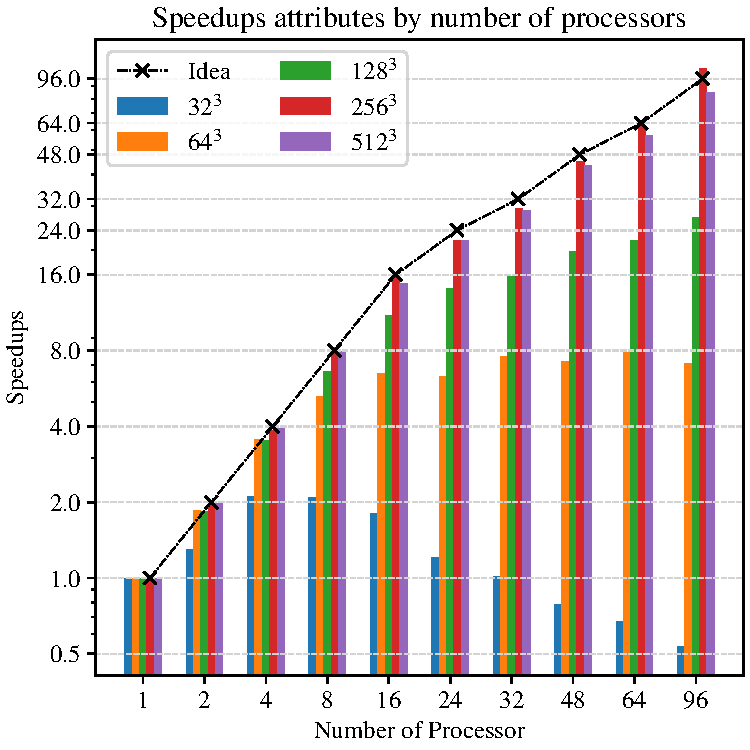
\includegraphics[width=0.45\textwidth]{figure/FIG_Benchmark_pure_mpi_3D.pdf}
    \label{FIG:Benchmark:Pure_MPI_Single_Node_3D}
  }
  \hfill
  \subfigure[Strong scaling on four node]
  {
    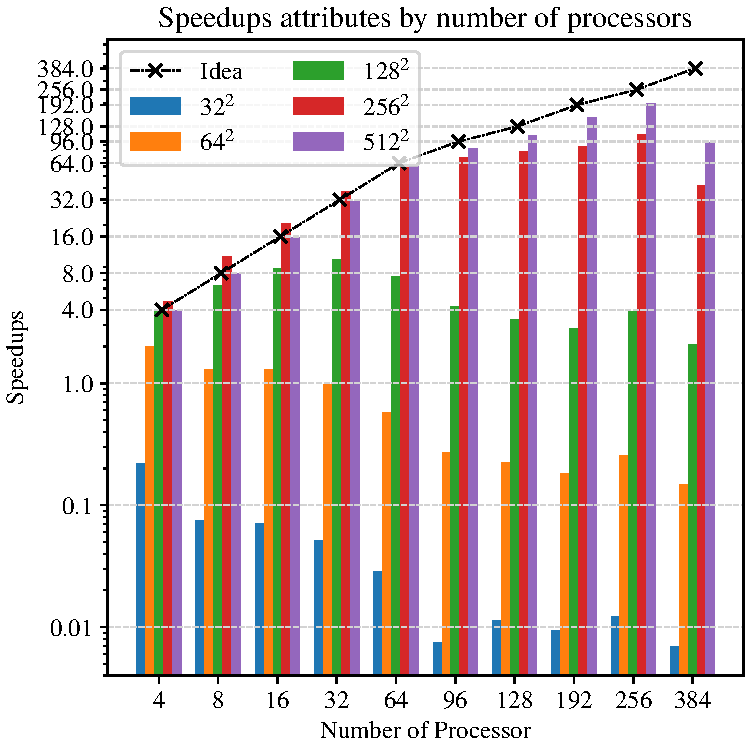
\includegraphics[width=0.45\textwidth]{figure/FIG_Benchmark_pure_mpi_3D_multi_nodes.pdf}
    \label{FIG:Benchmark:Pure_MPI_Multi_Node_3D}
  }
  \caption{
    Comparison of speedup ratios of strong scaling tests  pure MPI models on $4$ nodes of and $1$ node.
    The problem sizes are set to $32^3$, $64^3$, $128^3$, $256^3$ and $512^3$ and data type is \texttt{Double}.
  }
  \label{FIG:Benchmark:Pure_MPI_Node_3D}
\end{figure}

On the other hand, I specify the maximun scale of problem is $512^3$ rather than $1024^3$. 
This is because the pattern of accessing memories is $O(n^3)$ space complexity which leads more time consumption per epoch, 
although the problem has identical scale $1024^3 = 32768^2$. 
It also makes us harder to see a large superlinear speedup occurs comparing to 2D problems.
In this scenario, only the figure \ref{FIG:Benchmark:Pure_MPI_Multi_Node_3D} shows that the problem with scale $256^3$ has 
superlinear speedup on $8$, $16$ and $32$ CPUs due to the separated nodes has dependent CPU clock whic increase the rate of hitting cache.
\begin{figure}[htbp]
  \centering
  \subfigure[Single]{
    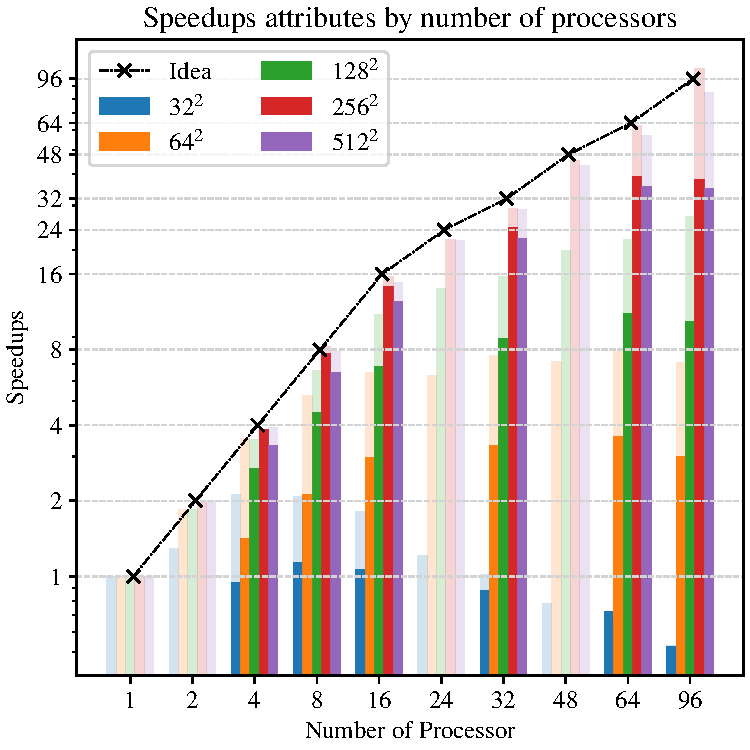
\includegraphics[width=0.38\textwidth]{figure/FIG_Benchmark_hybrid_0_single_nodes_3D.pdf}
    \label{FIG:Benchmark:FIG_Benchmark_hybrid_0_single_nodes_3D}
  }
  \hspace{0em} 
  \subfigure[Single]{
    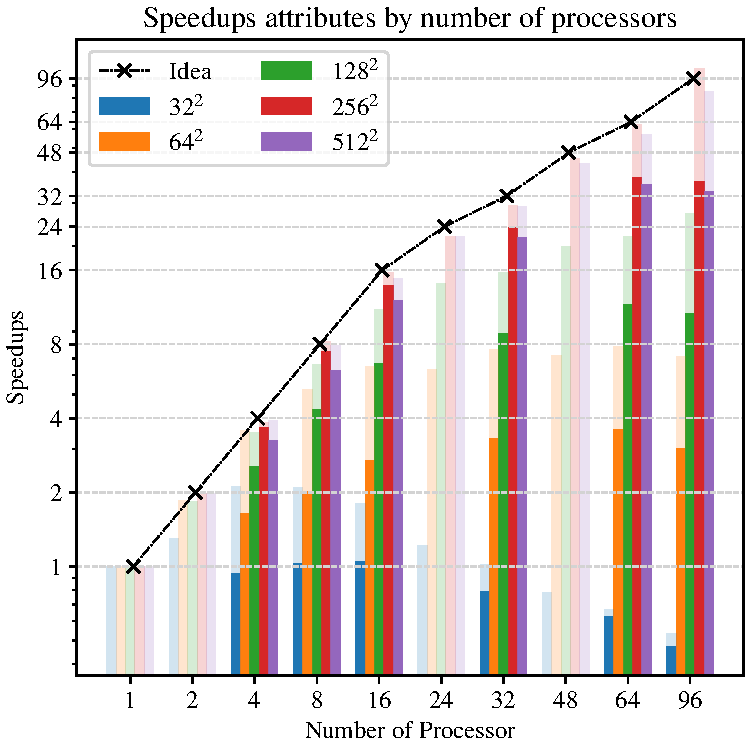
\includegraphics[width=0.38\textwidth]{figure/FIG_Benchmark_hybrid_1_single_nodes_3D.pdf}
    \label{FIG:Benchmark:FIG_Benchmark_hybrid_1_single_nodes_3D}
  }
  \hspace{0em} 
  \subfigure[caption]{
    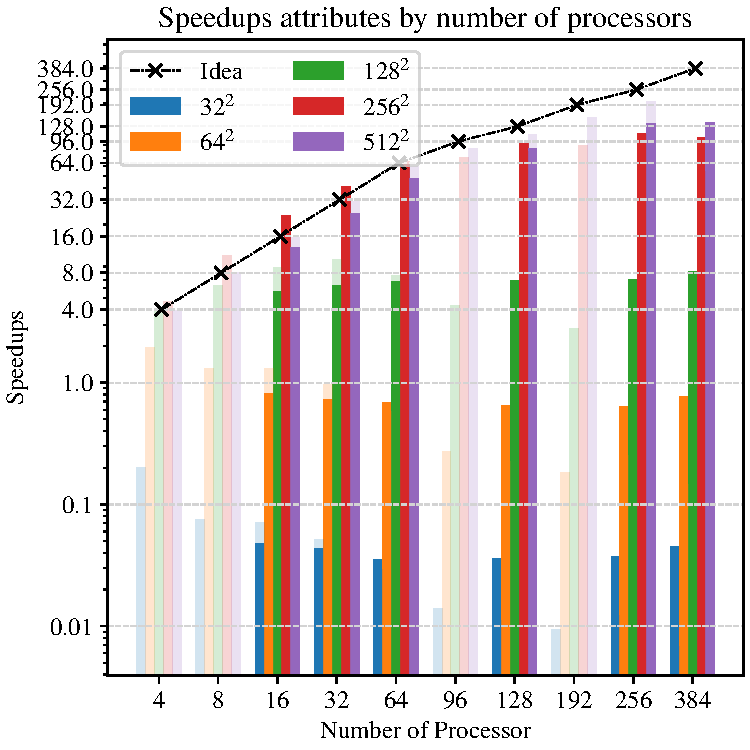
\includegraphics[width=0.38\textwidth]{figure/FIG_Benchmark_hybrid_0_multi_nodes_3D.pdf}
    \label{FIG:Benchmark:FIG_Benchmark_hybrid_0_multi_nodes_3D}
  }
  \hspace{0em} 
  \subfigure[caption]{
    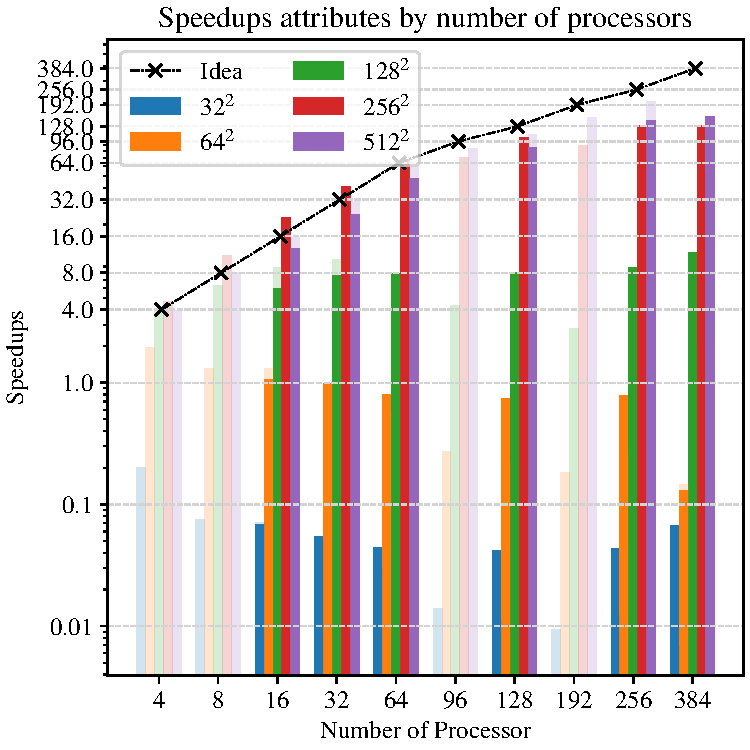
\includegraphics[width=0.38\textwidth]{figure/FIG_Benchmark_hybrid_1_multi_nodes_3D.pdf}
    \label{FIG:Benchmark:FIG_Benchmark_hybrid_1_multi_nodes_3D}
  }
  \caption{<caption>}
  \label{FIG:Benchmark:Hybrid_Single_Four_Node_3D}
\end{figure}

% \begin{wrapfigure}{r}{0.8\textwidth} 
%   \centering
%   \subfigure[Single]{
%     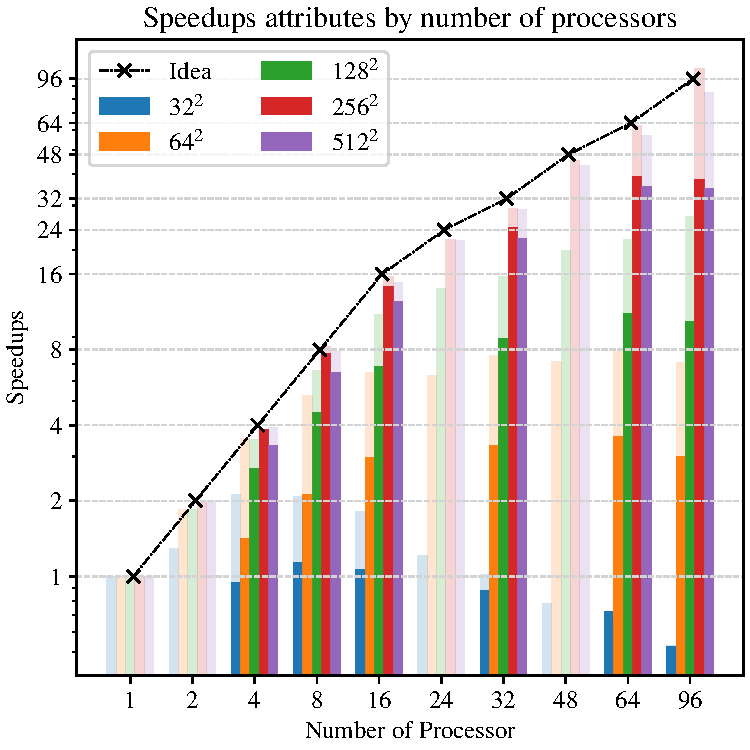
\includegraphics[width=0.35\textwidth]{figure/FIG_Benchmark_hybrid_0_single_nodes_3D.pdf}
%     \label{FIG:Benchmark:FIG_Benchmark_hybrid_0_single_nodes_3D}
%   }
%   \hspace{0em} 
%   \subfigure[Single]{
%     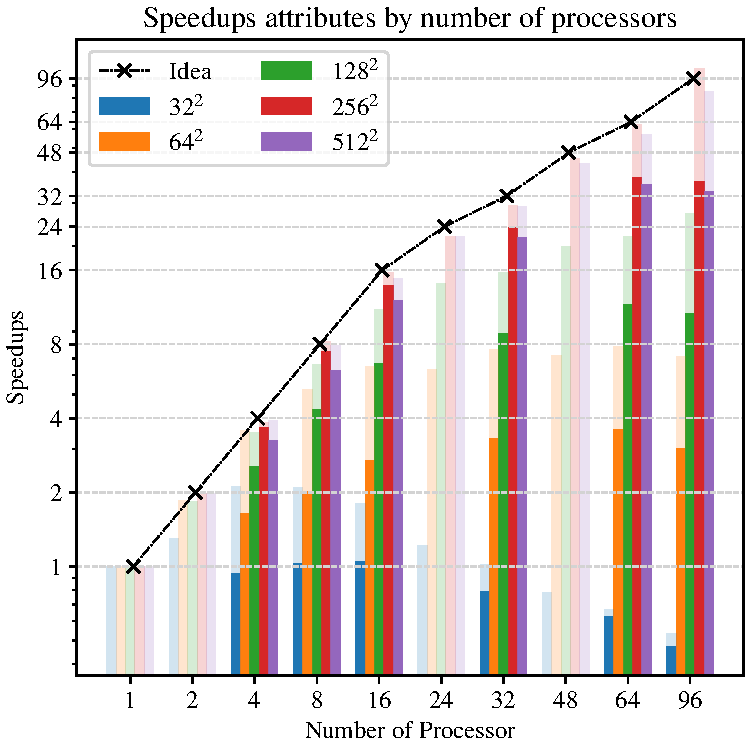
\includegraphics[width=0.35\textwidth]{figure/FIG_Benchmark_hybrid_1_single_nodes_3D.pdf}
%     \label{FIG:Benchmark:FIG_Benchmark_hybrid_1_single_nodes_3D}
%   }
%   \hspace{0em} 
%   \subfigure[caption]{
%     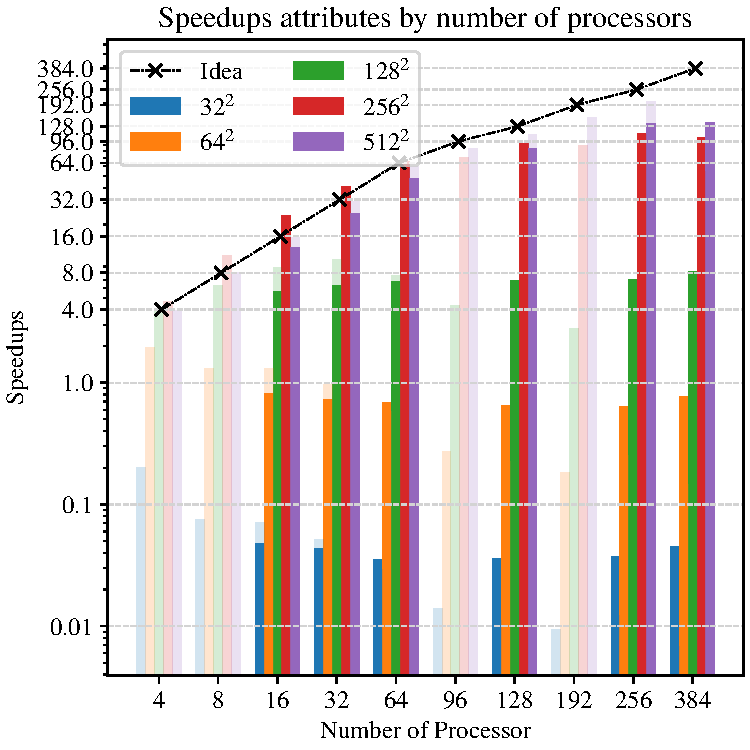
\includegraphics[width=0.35\textwidth]{figure/FIG_Benchmark_hybrid_0_multi_nodes_3D.pdf}
%     \label{FIG:Benchmark:FIG_Benchmark_hybrid_0_multi_nodes_3D}
%   }
%   \hspace{0em} 
%   \subfigure[caption]{
%     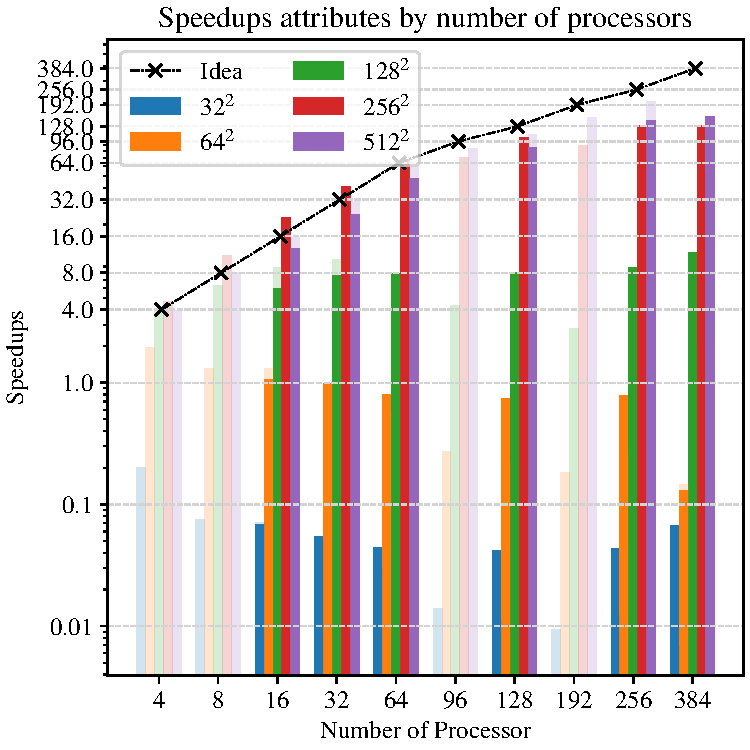
\includegraphics[width=0.35\textwidth]{figure/FIG_Benchmark_hybrid_1_multi_nodes_3D.pdf}
%     \label{FIG:Benchmark:FIG_Benchmark_hybrid_1_multi_nodes_3D}
%   }
%   \caption{<caption>}
%   \label{FIG:Benchmark:Hybrid_Single_Four_Node_3D}
% \end{wrapfigure}
The figure \ref{FIG:Benchmark:Hybrid_Single_Four_Node_3D} shows the details of hybrid parallel models on single and four nodes.
Overall, the figures \ref{FIG:Benchmark:FIG_Benchmark_hybrid_0_single_nodes_3D} and \ref{FIG:Benchmark:FIG_Benchmark_hybrid_1_single_nodes_3D}
show that both hybrid model have worse performance on single node. Even with the benefits of caching, the $256^3$ scale problem still 
a little bit loss on speedup on $4$, $8$ and $16$ CPUs.
However the figures \ref{FIG:Benchmark:FIG_Benchmark_hybrid_0_multi_nodes_3D} and \ref{FIG:Benchmark:FIG_Benchmark_hybrid_1_single_nodes_3D} 
shows completely different results.
On the multi-nodes test, overall, all hybrid models have better performance comparing to pure MPI parallelization.
Especially for the largest problem $512^3$ which the pure MPI scaling speedup ratio is $96$ under $384$ CPUs, the 
hybrid models gained approximately $130$ and $140$ speedups which is about $30\% ~ 40\%$ improvements.
Moreover, the problem with $256^3$ scale investigated on $8$ $16$ and $32$ CPUs reached superlinear speedup at the end,
which were making use of L3 cache and asynchronized CPU clock cycle.

As for the promotion gets from the cache and CPU asynchronization, we can discovered that the 2D problems got less benefits 
while the 3D problems got bigger.
This is the 3D problem relys more on the memory accessing, and the shared memory parallelization can do optimizations better than MPI.

\subsubsection{Weak Scaling}

The weak scaling results of 3 dimension problems are listed in the table \ref{TAB:Benchmark:Weak_3D_AllModels}.
For the single node scaling speedups, we could see that the pure MPI model has better performance over all problem scales 
and amount of resources.
However, for the multi-node tests, the hybrid models have approximately same or better performance than pue MPI model.
Especially for the non-overlapped hybrid model.


% pure_mpi 32 14.205280130981388 [9.07797386]
% pure_mpi 64 47.05604671282058 [30.1075974]
% pure_mpi 128 39.74555364101945 [25.42773957]

% hybrid_0 32 12.667882915956632 [8.09379942]
% hybrid_0 64 52.292330736249745 [33.45963735]
% hybrid_0 128 31.59871392899227 [20.21248921]

% hybrid_1 32 14.998693266535422 [9.58588224]
% hybrid_1 64 55.094846355099 [35.25368524]
% hybrid_1 128 31.416593371177605 [20.0959036]

\begin{table}[htbp]
  \caption{Weak Scaling of 3D Heat Equation}
  \label{TAB:Benchmark:Weak_3D_AllModels}
  \begin{minipage}{\columnwidth}
    \begin{center}
      \footnotesize % overleaf
      \begin{tabular}{>{\bfseries}p{2.5cm} p{1cm} p{1.5cm} p{1.5cm} p{1.5cm} p{1.5cm} p{1cm} p{1cm}}
        \toprule
        \multirow{2}{*}{Strategy} & \multirow{2}{*}{\bfseries Size} & \multicolumn{3}{c}{\bfseries  Number of CPUs}    & \multirow{2}{*}{\bfseries $f_p(\%)$}  & \multirow{2}{*}{\bfseries $f_p(\%)_{\text{Multi-node}}$}\\
                      &                      & \bfseries 8     & \bfseries 64        & \bfseries 64$_{\text{Multi-node}}$   &  &  &         \\
        \midrule
        Pure MPI      & \multirow{3}{*}{$32^3$}       & 5.243  & 26.405              &  9.078                     & 41.6 & 14.2 \\
        No Overlap    &                               & 2.124  & 13.386              &  8.094                     & 21.0 &  12.7\\
        With Overlap  &                               & 2.014  & 13.884              &  9.586                     & 21.8 & 39.7 \\
        \midrule
        Pure MPI      & \multirow{3}{*}{$64^3$}       & 7.937  & 32.034              &  30.106                    & 50.8 & 47.1 \\
        No Overlap    &                               & 5.393  & 20.007              &  33.460                    & 31.8 & 52.3 \\
        With Overlap  &                               & 5.200  & 19.558              &  35.254                    & 31.1 & 31.6 \\
        \midrule
        Pure MPI      & \multirow{3}{*}{$128^3$}      & 3.513  & 24.239              &  25.428                    & 38.0 & 39.7 \\
        No Overlap    &                               & 3.303  & 15.235              &  35.254                    & 24.1 & 55.1 \\
        With Overlap  &                               & 3.187  & 15.107              &  20.096                    & 23.9 & 31.4 \\
        \bottomrule
      \end{tabular}
    \end{center}
    % \bigskip
    % \footnotesize\emph{Source:} This is source 
  \end{minipage}
\end{table}

On the other hand, comparing the results from 2 dimension versions shown in table \ref{TAB:Benchmark:Weak_PURE_MPI} and \ref{TAB:Benchmark:Weak_PURE_MPI_Multi_Node}.
It is readily to determine that the weak scaling speedup of 3 dimension problems are worse than 2 dimensions.
Which means that the fraction of parallelizable parts in 3D problems are significantly lower than 2D version.


% \begin{wrapfigure}{r}{0.45\textwidth} 
%   \centering
%   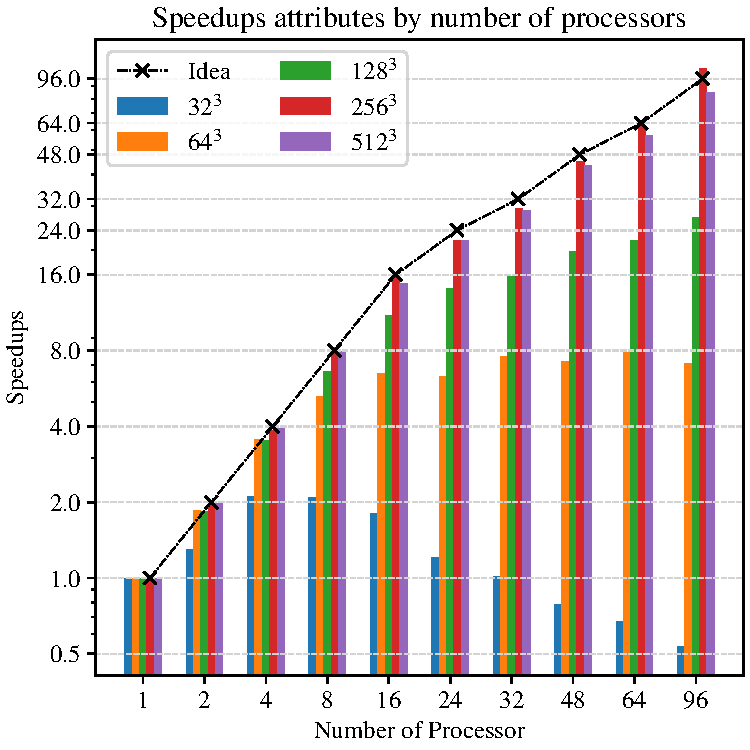
\includegraphics[width=0.5\textwidth]{figure/FIG_Benchmark_pure_mpi_3D.pdf}
%   \caption{
%     Comparison of speedup ratios of strong scaling tests of pure MPI parallelized program. 
%     % The investigated problem scales are the power of $2$, exponents ranging from $9$ to $15$.
%     % The number of CPUs are also set as power of $2$, with additional numbers $24$, $48$ and $96$ matched the topologies of CPU.
%   }
%   \label{FIG:Benchmark:PURE_MPI_3D}
% \end{wrapfigure}















\subsection{Comparison on Accuracy, with PINN}
Scalability is important for parallel computing to be effective, so as the quality of results.
In this section, the major comparison are about comparing the quality of numerical solutions of 
2D, 3D FDTD solvers and a state-of-art method PINN.


\subsubsection{Accuracy}
When we tried to represent numbers using arithmetic in binary, decimal or hexadecimal, truncation always affects the precision of every number, 
or so called as 
round-off-error.

\paragraph{Round-off Error}
In IEEE-754 \cite{IEEE_754} standards, a $32$-bit floating pointer number, single precision, obligatorily represented with $23$-bit mantissa, 
$8$-bit exponent and $1$-bit for sign. 
Where as $64$-bit floating number, double precision, also ubiquitous used, which has $11$-bit exponent and $52$-bit mantissa.
After almost three decades development, not only single and double precisions (float32, float64) are ubiquitously in use, 
also more formats such as fp4, fp8, and fp16 etc. Both of them follows the simple form of exponent $k$, sign $n$ and mantissa $N$. 
\cite{IEEE_754_p2_eq1}
\begin{equation*}
  2^{k+1-N}n
\end{equation*}
Round-off errors are a manifestation of the fact that on a digital computer, which is unavoidable in numerical computations.
In such case, the precision of the number depends on how many bytes are used to store single number. 
For instance, a float32 number provides $2^{-23} \approx 1.2\times10^{-7}$, and a double precision number gives $2^{-53} \approx 2.2\times10^{-16}$, 
such number is called machine $\epsilon$ which is the smallest number the machine can represent with given format.

In numerical methods I investigated, the FDTDs are conventionally using double precision number so that the programs can treat extreamly large and small 
numbers simultaneously in the same computation, without worring about the round-off errors.
However, as mentioned, fp32 and fp16 are also popular use in scientific computing, especially in machine learning training process. 
While the lasted training GPUs are integrated compute accelarate unit for low precision floating numbers. \cite{NVIDIA_HB200_PAPER}.

\paragraph{Floating-point Arithmetic}
The other type loss comes from the arithmetic operations on two numbers $x$, $y$. 
The standard model holds that 
\begin{equation}
  fl(x \:\text{op}\: y) = (x \: \text{op} \: y) (1+\delta), \:\:\: \left|\delta\right| < \epsilon
\end{equation}
where the $op$ stands for the four elementary operations: $+, -, \times, /$. \cite{Germund,NMSC,V1,P112}.




% \subsection{Finite Difference Methods}
% \subsubsection{Pure Message Passing Parallel}
% \subsubsection{Hybrid Parallel}


% \subsection{Physics Informed Neural Networks}
% \subsubsection{CUDA parallel}
% \subsubsection{Hybrid Parallel}


% \subsection{Visualization}


% \subsection{Comparison on Boundary Conditions}










% Table 
% lists the results 

% \begin{table}
%   \caption{Strong Scaling on Single Node of 2D Heat Equation}
%   \label{}
%   \begin{minipage}{\columnwidth}
%     \begin{center}
%       \begin{tabular}{lcccccc}
%         \toprule
%         Scale & $1024^2$ & $2048^2$ & $4096^2$  & $8192^2$  & $16384^2$ & $32768^2$\\
%         \midrule
%         2     & 1        & 1        &   1       & 1         & 1         & 1 \\
%         4     & 1        & 1        &   1       & 1         & 1         & 1 \\
%         8     & 1        & 1        &   1       & 1         & 1         & 1 \\
%         16     & 1        & 1        &   1       & 1         & 1         & 1 \\
%         32     & 1        & 1        &   1       & 1         & 1         & 1 \\
%         48     & 1        & 1        &   1       & 1         & 1         & 1 \\
%         64     & 1        & 1        &   1       & 1         & 1         & 1 \\
%         96     & 1        & 1        &   1       & 1         & 1         & 1 \\
%         \bottomrule
%       \end{tabular}
%     \end{center}
%     % \bigskip
%     % \footnotesize\emph{Source:} This is source 
%   \end{minipage}
% \end{table}